\subsection{Жироскоп и Акселерометър}
\FloatBarrier

Изпозван е чип \textit{LSM6DS33} (\autoref{fig:acc_gyro_directions_and_pinout}) \cite{accgyrorefman},
който е интегрирано пакетно решение, 
предоставящо 3D дигитален Жироскоп и 3D дигитален акселерометър.
Чипът използва \(1.7 \to 3.6V\) захранване катo в нужният ни решим се нуждае от \(0.9mA\).
Чипът е част от сензорна платка, позволяваща директна връзка чрез протокол \textit{I2C} (адрес: \texttt{0xD6}).


За целите на настоящият ни проект е използвана следната конфигурация:
Използва се директен достъп (без буфериране) до измерените стойности.
Обхват на Акселерометъра \(\pm 8g\), Обхват на Жироскопа \(\pm 1000 dps\).


\begin{figure}[htpb!]
    \centering
    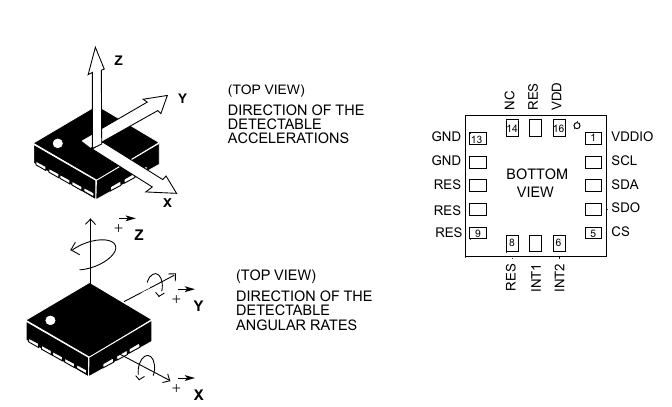
\includegraphics[width=0.7\textwidth]{acc_gyro_directions_and_pinout}
    \caption{\textit{LSM6DS33} Ориентация на осите и наименованията на пиновете в пакета}
    \label{fig:acc_gyro_directions_and_pinout}
\end{figure}

\FloatBarrier